\documentclass[10pt,letterpaper]{article}
\usepackage[T1]{fontenc}
\usepackage{lmodern}
\usepackage[margin=0.87in]{geometry}
\usepackage{amsmath,amssymb,amsthm,booktabs,graphicx,array}
\usepackage[hidelinks]{hyperref}
\graphicspath{{../output/}{output/}{figures/}{docs/figures/}}
\setlength{\parindent}{0pt}
\setlength{\parskip}{5pt}
\setlength{\emergencystretch}{2em}
\newcounter{projectalgorithm}
\newenvironment{algorithmbox}[2]
  {\par\medskip\noindent
   \begin{minipage}{\linewidth}
   \refstepcounter{projectalgorithm}\label{alg:#1}%
   \hrule height 0.6pt\relax\smallskip
   \noindent\textbf{Algorithm \theprojectalgorithm.\ #2}\par\smallskip
   \hrule\smallskip\small\setlength{\parskip}{3pt}%
   \setlength{\abovedisplayskip}{4pt}\setlength{\belowdisplayskip}{4pt}%
   \setlength{\abovedisplayshortskip}{3pt}\setlength{\belowdisplayshortskip}{3pt}%
   \let\projectenumerate\enumerate
   \renewcommand{\enumerate}{\projectenumerate
     \setlength{\itemsep}{2pt}\setlength{\parsep}{0pt}}%
  }
  {\par\smallskip\hrule height 0.6pt\relax\end{minipage}\par\medskip}
\newcommand{\costsummary}[1]{\noindent{\small\textbf{Big-O summary.} #1}\par}
\newtheorem{theorem}{Theorem}
\newtheorem{proposition}{Proposition}
\renewcommand{\qedsymbol}{\rule{0.68ex}{0.68ex}}
\newenvironment{proofsteps}{%
  \setlength{\abovedisplayskip}{4pt}%
  \setlength{\belowdisplayskip}{4pt}%
  \setlength{\abovedisplayshortskip}{3pt}%
  \setlength{\belowdisplayshortskip}{3pt}%
  \begin{list}{\arabic{enumi}.}{\usecounter{enumi}%
    \setlength{\leftmargin}{1.45em}\setlength{\labelsep}{0.4em}%
    \setlength{\topsep}{2pt}\setlength{\itemsep}{2pt}%
    \setlength{\parsep}{0pt}\setlength{\partopsep}{0pt}}%
}{\end{list}}
\hypersetup{pdftitle={Curvature, Energy, and Collisions in Nonconvex Optimization},pdfauthor={Yit Xiaang Ztang}}

\begin{document}
\begin{center}
{\small EE 5239 \quad Introduction to Nonlinear Optimization \quad Fall 2026}\\[9pt]
{\LARGE\bfseries Curvature, Energy, and Collisions\\[3pt] in Nonconvex Optimization}\\[8pt]
{\large Yit Xiaang Ztang}\\
Individual course project
\end{center}

\begin{abstract}
This project asks when redistributing momentum helps a search cross a barrier and when it disturbs a good solution. Early trials showed that reflecting uphill steps could prevent escape. In a held-out double-well comparison, collision search with a settling phase finished at the target in \(14/20\) runs, compared with \(0/20\) for four-start Momentum and \(16/20\) for conservation-matched random scattering. In a separate test, lowering bounce height and transferring horizontal momentum protected an already good particle. For a vertical orbit above a quadratic minimum, I prove that the undamped linearized return is bounded exactly when \(0<\kappa H<1/2\), where \(\kappa\) is wall curvature and \(H\) is bounce height. On NanoGPT, conservative velocity exchange lowered the first post-exchange training loss on average, but raised mean final test loss by \(0.01879\) relative to independent Momentum SGD replicas. AdamW had the lowest test loss in all ten seed groups.
\end{abstract}

\section{Problem and modeling choices}

Momentum can carry an iterate across a region of high loss and help it escape a poor basin. The same motion can carry an already good iterate out of its basin. I chose collisions as a model because they offer a way to redistribute a fixed pool of kinetic energy among search trajectories. I test how the direction of that transfer, the energy kept by the current best particle, and the timing of damping affect basin crossing and settling. I track the active particle that starts near the good minimum separately from the historically best point saved for delivery.

\paragraph{Trial-step reflection.}
The proposal used Polyak's heavy-ball momentum \cite{polyak}, \(u_i=\beta v_i-\eta\nabla f(x_i)\). The original rule reflected a trial direction if uphill motion and a sufficient loss increase persisted. With unit gradient normal \(n\) and restitution \(e\), it used \(u_i^+=u_i-(1+e)(u_i^\top n)n\). In the double-well pilot, plain Momentum succeeded in \(6/10\) runs, while both reflection and momentum reset succeeded in \(0/10\). Both interventions helped precision on the pilot quadratic. A step directed uphill can overshoot a good minimum or carry the search toward a separating barrier. The pilot prompted a model in which wall contact determines reflection. Adaptive restart provides a related baseline \cite{restart}.

\paragraph{Gravity and wall contact.}
The gravity simulator has its own equations of motion. It adds a height \(z\) and constrains \(z\ge f(x)\). In free flight, horizontal velocity is constant and \(\ddot z=-g\). The solver locates the first incoming root of \(z(t)-f(x(t))\) using the analytic loss along the horizontal path. At contact \(V^+=V^--2(V^-\cdot n)n\), where \(n=(-\nabla f,1)/\sqrt{1+\|\nabla f\|^2}\). The solver then advances the remaining time. The fixed wall supplies an external impulse and preserves kinetic energy at contact. In free flight, \(K+gz\) is constant for unit mass. The imposed damping \(V\leftarrow \beta V\) removes \((1-\beta^2)K\). Algorithm~\ref{alg:gravity} gives the event loop.

\paragraph{Pair collisions and a matched control.}
For two equal masses, write \(c=(V_i+V_j)/2\) and \(w=(V_i-V_j)/2\). At an approaching encounter the normal rule reflects \(w\) about the contact plane. A comparison rule draws \(w^+\) from the outgoing hemisphere at the same encounter. Both preserve \(c\) and \(\|w\|\), hence pair linear momentum and kinetic energy. The energy change for particle \(i\) is \(c\cdot(w^+-w^-)\), with the opposite change for \(j\). The central normal impulse preserves pair angular momentum at the event. The random control generally changes it, and the two rules can lead to different later encounters.

\clearpage
\section{Algorithms and implementation}
\label{sec:algorithms}

Algorithm~\ref{alg:gravity} resolves contacts on analytic landscapes. Algorithms~\ref{alg:damping} and~\ref{alg:swap} modify native Momentum SGD. Algorithm~\ref{alg:external} keeps the base optimizer's statistics local and exchanges a separate displacement. Appendix~\ref{app:algorithms} gives the computational costs.

In the summaries, \(P\) counts particles or replicas, \(d\) is the dimension per particle or model, \(T\) counts updates per replica, and \(J\) counts pair swaps. \(C_{\rm wall}\) is the cost of one wall search and \(C_\nabla\) of one minibatch gradient. Training overhead is relative to the same base optimizer and replica count.

\begin{algorithmbox}{gravity}{Gravity-driven particle search}
\textbf{Input.} Feasible states \((x_i,z_i,V_i)\), wall \(f\), gravity \(g>0\), observation interval \(h\), damping rule, pair contact rule, and stopping budget.
\begin{enumerate}
\item \textbf{Initialize.} Evaluate the initial losses and initialize the historical best.
\item \textbf{Simulate.} While the budget permits another observation interval
  \begin{enumerate}
    \item Apply the specified damping and set remaining time \(r\gets h\).
  \item While \(r>0\), find the earliest incoming wall or enabled pair contact within \(r\). Advance all particles by ballistic motion to that event, or by \(r\) if there is no event. Deduct the elapsed time and, for a contact, apply the corresponding update:
  \[
  \begin{aligned}
  \text{wall:}\quad &V_i^+=V_i^--2(V_i^-\!\cdot n)n,\\
  \text{pair:}\quad &(V_i^+,V_j^+)=(c+w^+,c-w^+),
    \qquad c=(V_i^-+V_j^-)/2 .
  \end{aligned}
  \]
  Here \(n\) is the unit wall normal, and the pair contact rule selects \(w^+\).
  \item At the saved observation, record current losses and update the historical best. Charge function, gradient, and path queries as they occur.
  \end{enumerate}
\item \textbf{Output.} \textbf{Return} the historical best point and the trajectory and cost summaries when the stopping condition is reached.
\end{enumerate}
\end{algorithmbox}
\costsummary{Each pass costs \(O(PC_{\rm wall}+P^2d)\), with pair checks added to independent gravity search.}

\begin{algorithmbox}{damping}{State-dependent Momentum SGD on NanoGPT}
\textbf{Input.} Initial parameters \(\theta_0\), training minibatch stream, step size \(\eta\), momentum \(0.9\), gradient clipping norm \(C\), update budget \(T\), and control scale \(a_\star\) (\(0.5\) for damping or \(0\) for reset). Use zero weight decay.
\begin{enumerate}
\item \textbf{Initialize.} Set inherited displacement \(u_0=0\), with empty warning history and zero actions.
\item \textbf{Update.} For \(t=0,\ldots,T-1\)
  \begin{enumerate}
  \item Draw the next minibatch and compute the clipped gradient \(g_t\). Flag the update if both vectors are nonzero and
  \[
  \cos(u_t,g_t)>0.1,\qquad
  \|u_t\|>2\eta\|g_t\|,\qquad
  \frac{\|u_t\|}{1+\|\theta_t\|}>10^{-3}.
  \]
  \item Set \(a_t\gets1\). \textbf{If} at least two of the latest three updates are flagged, the 10-update cooldown has elapsed, and fewer than 20 actions have fired, set \(a_t\gets a_\star\), record the action, and clear the warning history.
  \item Update \(u_{t+1}\gets0.9a_tu_t-\eta g_t\) and \(\theta_{t+1}\gets\theta_t+u_{t+1}\).
  \end{enumerate}
\item \textbf{Output.} \textbf{Return} the final parameters \(\theta_T\) and evaluate their test loss.
\end{enumerate}
\end{algorithmbox}
\costsummary{Training costs \(O(T(C_\nabla+d))\), including \(O(Td)\) extra for norm checks and buffer scaling.}

The fixed-schedule control scales the native buffer by \(0.5\) after steps 80, 160, 240 and 320. The comparison used \(T=400\) updates.

\clearpage
\begin{algorithmbox}{swap}{Momentum SGD with scheduled velocity exchange}
\textbf{Input.} Four initial states and batch streams \((\theta_{i,0},\mathcal B_i)_{i=0}^3\), step size \(\eta\), momentum \(\mu\), clipping norm \(C\), local budget \(T\), disjoint pair matchings \((\mathcal M_t)_{t=1}^T\) (empty at unscheduled steps), and validation loss \(L_{\rm val}\).
\begin{enumerate}
\item \textbf{Initialize.} Set \(u_{i,0}^{+}=0\) for all \(i\).
\item \textbf{Update and exchange.} For \(t=1,\ldots,T\)
  \begin{enumerate}
    \item \textbf{For each} replica \(i\), draw \(B_{i,t}\) from \(\mathcal B_i\). Set
  \(\tilde g_{i,t}=\nabla_\theta\ell(\theta_{i,t-1};B_{i,t})\) and
  \(g_{i,t}=\tilde g_{i,t}\min\{1,C/(\|\tilde g_{i,t}\|+10^{-6})\}\). Update
  \[
    u_{i,t}^{-}=\mu u_{i,t-1}^{+}-\eta g_{i,t},
    \quad \theta_{i,t}=\theta_{i,t-1}+u_{i,t}^{-},
    \quad u_{i,t}^{+}=u_{i,t}^{-}.
  \]
  \item \textbf{For each} \((i,j)\in\mathcal M_t\), set
  \((u_{i,t}^{+},u_{j,t}^{+})=(u_{j,t}^{-},u_{i,t}^{-})\).
  \end{enumerate}
\item \textbf{Output.} \textbf{Return} \(\theta_{\hat i,T}\), where
\(\hat i=\min\operatorname*{arg\,min}_{0\le i\le 3} L_{\rm val}(\theta_{i,T})\).
\end{enumerate}
\end{algorithmbox}
\costsummary{Training costs \(O(PT(C_\nabla+d)+Jd)\), with \(O(Jd)\) added for audited velocity swaps.}

\begin{algorithmbox}{external}{SGD or Adam-family updates with external velocity exchange}
\textbf{Input.} Optimizer type, initial parameters and auxiliary displacements \(q_{i,0}\) for \(P\) replicas, training streams, validation loss, step size \(\eta>0\), auxiliary damping \(0\le\rho<1\), matched pairs and optional impulses \(J_{i,t}\), and update budget \(T\). For guarded mode use \(L>0\) and \(\eta\le1/L\). Zero initialization is the default for \(q\). A nontrivial exchange requires unequal auxiliary displacements, produced by initialization or an impulse.
\begin{enumerate}
\item \textbf{Initialize.} Initialize the optimizer buffers to zero. For Adam or AdamW choose \(\beta_1,\beta_2\in[0,1)\) and \(\epsilon_{\rm A}>0\). Use \(\lambda\ge0\) for AdamW's decoupled weight decay. For coupled regularization in Adam, include its penalty in the objective whose gradient is supplied.
\item \textbf{Propose, exchange, and test.} For \(t=0,\ldots,T-1\)
  \begin{enumerate}
    \item Compute each gradient estimate \(G_i\) at \(x_{i,t}\), with clipping if configured. For SGD let \(b_i=-\eta G_i\). For Momentum SGD update \(v_i\gets\mu v_i-\eta G_i\) and let \(b_i=v_i\). For Adam and AdamW, update the local moments and compute
  \[
  \begin{aligned}
  m_i&\gets\beta_1m_i+(1-\beta_1)G_i,\qquad
  w_i\gets\beta_2w_i+(1-\beta_2)G_i^{\odot2},\\
  \widehat m_i&=m_i/(1-\beta_1^{t+1}),\qquad
  \widehat w_i=w_i/(1-\beta_2^{t+1}),\\
  b_i&=-\eta\,\widehat m_i/(\sqrt{\widehat w_i}+\epsilon_{\rm A}).
  \end{aligned}
  \]
  Division and square roots act coordinatewise. For AdamW subtract \(\eta\lambda x_{i,t}\) from \(b_i\) for coordinates subject to decay.
  \item Form \(r_i=q_{i,t}+J_{i,t}\), with \(J_{i,t}=0\) if unsupplied. Swap the \(r_i\)'s in each scheduled disjoint pair, keeping network parameters and local optimizer buffers fixed. Set \(q_{i,t+1}=\rho r_i\) using the resulting \(r_i\). Record supplied impulses and damping separately from the exchange.
  \item Propose \(d_i=b_i+q_{i,t+1}\). In guarded mode keep it only if
  \[
    G_i^\top d_i+\tfrac L2\|d_i\|^2\le-\tfrac\eta2\|G_i\|^2
    \quad\text{and}\quad
    \|d_i\|\le2\eta\|G_i\|.
  \]
  A failed test gives \(d_i=-\eta G_i\). Set \(x_{i,t+1}=x_{i,t}+d_i\), keep the buffers computed in (a), and advance the step counter once.
  \end{enumerate}
\item \textbf{Output.} \textbf{Return} the lowest validation-loss replica for evaluation, breaking ties by index. Record the swap, impulse, and fallback counts.
\end{enumerate}
\end{algorithmbox}
\costsummary{Training costs \(O(PT(C_\nabla+d)+Jd)\), with \(O(PTd+Jd)\) added for auxiliary steps, swaps and checks.}

\paragraph{External velocity exchange for Adam and AdamW.}
Adam \cite{adam} uses the first moment divided by a coordinatewise scale from the second moment. Swapping raw first moments between replicas with different scales can change the sum and squared norms of the resulting parameter displacements. Algorithm 4 instead exchanges an auxiliary displacement expressed in parameter units. Each replica updates its own optimizer state from its own gradient. The NanoGPT trial used one replica and the unguarded impulse. Pair exchange and the descent safeguard are proposed extensions.

Without supplied impulses, \(q_{i,0}=0\) gives \(q_{i,t}=0\) for all \(t\).

\clearpage
\section{Local analysis of the vertical bounce}
\label{sec:analysis}

\begin{theorem}[Stability of the linearized bounce]\label{thm:bounce}
Let a unit-mass particle move under constant gravity \(g>0\) above the fixed wall \(f(x)=\kappa x^2/2\), with \(\kappa>0\). Assume elastic wall reflections, zero drag, and no other impulses. On the energy surface \(gH\) with \(H>0\), the vertical orbit at \(x=0\) has a linearized return map whose iterates are bounded for every initial perturbation if and only if \(0<\kappa H<1/2\).
\end{theorem}

\begin{proof}
\begin{proofsteps}
\item \textit{First return time.} Write the initial state just after reflection as \((x,u)\) with upward speed \(w\). Set \(v=\sqrt{2gH}\) and \(T=2v/g\). Energy conservation and the ballistic trajectory give
\[
\begin{aligned}
w&=\sqrt{v^2-g\kappa x^2-u^2},\\
z(t)-f(x+ut)&=t\left(w-\kappa xu-\tfrac12(g+\kappa u^2)t\right).
\end{aligned}
\]
Near \((0,0)\), the radicand is positive and \(w-\kappa xu>0\) by continuity. The gap is positive for \(0<t<t_*\), where \(t_*=2(w-\kappa xu)/(g+\kappa u^2)\). Its time derivative at \(t_*\) is \(-(w-\kappa xu)<0\), so this root is an incoming contact. At the orbit \(t_*=T\). Since the derivatives of \(x^2,xu,u^2\) vanish there, \(D_0w=D_0t_*=0\).
\item \textit{Reflection.} Set \(X=x+t_*u\), \(W=w-gt_*\), and \(s=\kappa X\). The unit normal is \(n=(-s,1)/\sqrt{1+s^2}\). Thus
\[
U=u-2\big((u,W)\cdot n\big)n_x=u+s\frac{2(W-su)}{1+s^2}.
\]
At the orbit \(u=s=0\) and \(W=-v\). By the product rule, \(D_0(t_*u)=T\,du\), and only the derivative of \(s\) contributes to the reflection term in \(U\), with coefficient \(-2v\). Hence \(D_0X=dx+T\,du\) and \(D_0U=du-2v\kappa D_0X\). In the coordinates \((x,u)\) this gives
\[
M=\begin{pmatrix}1&T\\-2v\kappa&1-2v\kappa T\end{pmatrix},
\qquad \det M=1,\quad \tau:=\operatorname{tr}M=2-8\kappa H.
\]
\item \textit{Boundedness for \(|\tau|<2\).} Set \(y=x+Tu\), so \(u=(y-x)/T\). The linearized update is \(x'=y,\ u'=u-2v\kappa y\). Thus \(y'=x'+Tu'=\tau y-x\). The polynomial is \(s^2-\tau s+1\). When \(|\tau|<2\) its roots have modulus one. To bound the iterates, define \(Q(x,y)=x^2+y^2-\tau xy\). Substitution and completion of the square give
\[
\begin{aligned}
Q(y,\tau y-x)&=y^2+(\tau y-x)^2-\tau y(\tau y-x)=Q(x,y),\\
Q(x,y)&=(y-\tau x/2)^2+(1-\tau^2/4)x^2.
\end{aligned}
\]
By symmetry, \(Q\) also bounds \((1-\tau^2/4)y^2\). The invariant \(Q(x_n,y_n)=Q(x_0,y_0)\) therefore bounds \(x_n,y_n\), and hence \(u_n\).
\item \textit{Unboundedness for \(\tau\le-2\).} For \(\tau<-2\), the smaller root \(\lambda=(\tau-\sqrt{\tau^2-4})/2\) is below \(-1\). Since \(\tau\lambda-1=\lambda^2\), the update sends \((1,\lambda)\) to \(\lambda(1,\lambda)\), giving \(x_n=\lambda^n\). For \(\tau=-2\), put \(a=2v\kappa\). Then \(aT=4\) and
\[
N=M+I=\begin{pmatrix}2&T\\-a&-2\end{pmatrix}\ne0,\qquad
N^2=(4-aT)I=0.
\]
In \(M^n=(-I+N)^n\), all terms of degree at least two in \(N\) vanish. Thus \(M^np=(-1)^n(p-nNp)\), and \(p=(0,1)\) gives \(|(M^np)_1|=nT\). Since \(g,H,\kappa>0\) imply \(\tau<2\), the bounded case is exactly \(0<\kappa H<1/2\). \qedhere
\end{proofsteps}
\end{proof}

The trace agrees with Dullin's gravitational billiard formula \cite[Sec.~5]{dullin} at energy \(gH\). Lean 4 checks the first incoming contact, differentiation of the exact reflected return and the boundedness classification, including growth at \(\kappa H=1/2\).

A flat mode is a shear. For a \(C^2\) wall at a minimum \(x_\star\), the vertical return is transverse since the normal speed there is \(-v\ne0\). The local return time is differentiable by the implicit function theorem. The derivative of the horizontal motion is \(dX=dx+T\,du\), and the derivative of the normal slope is \(B\,dX\) for \(B=\nabla^2f(x_\star)\), giving \(dU=du-2vB\,dX\). For \(B\succ0\) its orthogonal eigenbasis splits the Jacobian into the scalar blocks above, giving \(H\lambda_{\max}(B)<1/2\). The extension is a statement about the linearized orbit. Protection over finite nonlinear excursions requires a bound on the remainder of the return map.

\paragraph{Connection to course algorithms.}
Gradient descent contracts on a quadratic mode when \(|1-\eta\kappa|<1\). The bounce recurrence \(x_{n+2}=(2-8H\kappa)x_{n+1}-x_n\) is quadratic heavy-ball with unit momentum and effective step \(8H\). In the stable range its preserved quadratic quantity allows persistent oscillations.

\clearpage
\section{Evidence from the synthetic landscapes}

\paragraph{Numerical check of the return map.}
In a parabolic-wall sweep, three curvatures \(\kappa=1,4,16\) were crossed with ten values of \(\kappa H\). Central differences at perturbation sizes \(10^{-6}\) and \(10^{-7}\) on a fixed energy surface with \(g=0.5\) yielded 60 Jacobians from 270 return probes. Their maximum absolute entrywise discrepancy from the analytic matrices was \(3.91\times10^{-9}\). The measured trace was \(-1.92\) at \(\kappa H=0.49\) and \(-2.08\) at \(0.51\) to two decimal places.

\begin{figure}[htbp]
\centering
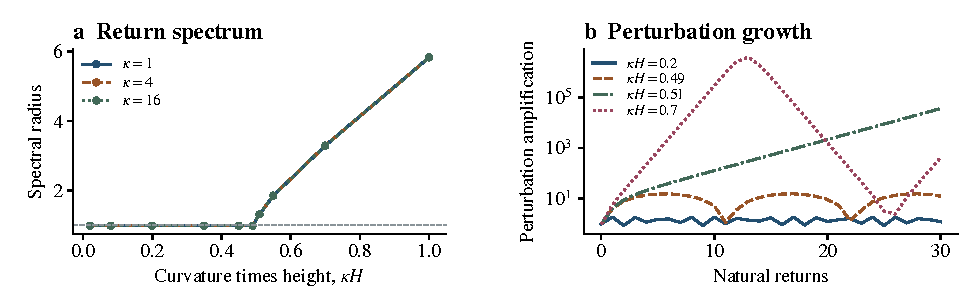
\includegraphics[width=0.96\linewidth]{bounce_stability.pdf}
\caption{Parabolic-wall sweep. \textbf{a} Spectral radius of the measured one-bounce Jacobian. \textbf{b} Disturbance amplification along 30-bounce trajectories at curvature 4. The linearized condition bounds the powers of the return map and still permits transient growth.}
\end{figure}

\paragraph{Rosenbrock.}
The largest local curvature in a rotated 2D Rosenbrock test was approximately \(20.032\). The table shows one particle perturbed by \(10^{-8}\) in that direction, run for physical time 25 with step 0.0125. At \(H=0.08\), a run without the deliberate perturbation reached a peak rise of only \(6.60\times10^{-18}\). The perturbed run exposes sensitivity that the near-symmetric run misses.

\begin{center}
\begin{tabular}{@{}rrrr@{}}
\toprule
Initial \(H\) & \(20.032H\) & Peak loss rise & Final loss rise\\
\midrule
0.002 & 0.0401 & \(1.00\times10^{-15}\) & \(3.00\times10^{-19}\)\\
0.020 & 0.4006 & \(4.06\times10^{-15}\) & \(3.05\times10^{-20}\)\\
0.080 & 1.6026 & \(7.38\times10^{-3}\) & \(3.37\times10^{-6}\)\\
\bottomrule
\end{tabular}
\end{center}
This finite-time test uses damping and a nonlinear, anisotropic wall. The small rises at the two lower heights and the larger rise at the highest shown height are consistent with the undamped local boundary. The analysis applies to the linearized return map. Peak size and crossing time are empirical measurements here.

\paragraph{Height allocation with matched energy.}
In the height-allocation study, I estimated the largest local eigenvalue with paid central gradient probes and assigned the current best particle
\[
 H_j=\min\left(0.8,\,0.2/\max(\widehat\lambda_j,10^{-6})\right).
\]
When the cap binds, the estimated curvature times height is 0.2. I gave the unused height to the other three particles so the group started with the same total energy. The explorers started in motion because the at-rest controls had no hits. The good particle started at rest. At stiffness \(1,8,32\), runs with a rise above \(10^{-4}\) in the good particle's loss fell from \(19/20,20/20,20/20\) to zero at every stiffness. In separate runs with all particles in the poorer basin, final hits moved from \(17/20,10/20,8/20\) to \(16/20,10/20,7/20\).

The cap gives the good particle a shorter bounce and leaves energy for the others to search. Its clearest benefit was keeping the loss of an already good point close to its starting value. When the group had to find the better basin from scratch, this allocation made little difference to how often it finished at the target.

\clearpage
\paragraph{Separating height from horizontal momentum.}
In the height and momentum ablation, eight allocations shared the same initial total energy and linear momentum within each paired context. The transfer sets the selected particle's horizontal velocity to zero, shifts the other velocities to retain total linear momentum, and rescales their relative velocities to restore group kinetic energy. The transformation generally changes angular momentum. The particles then move independently with wall reflections and damping. The departure columns count runs in which the saved incumbent loss rose by more than \(10^{-4}\) above its initial value.

\begin{center}
\small
\begin{tabular}{@{}lrrrr@{}}
\toprule
 & \multicolumn{2}{c}{Height times transverse curvature}
 & \multicolumn{2}{c}{Incumbent departures}\\
\cmidrule(lr){2-3}\cmidrule(l){4-5}
Initialization & \(\kappa=8\)& \(\kappa=32\)& \(\kappa=8\)& \(\kappa=32\)\\
\midrule
Fixed \(H=0.025\), transfer & 0.20 & 0.80 & 0/20 & 20/20\\
Fixed \(H=0.00625\), transfer & 0.05 & 0.20 & 0/20 & 0/20\\
Curvature cap, keep velocity & \(\approx0.20\)&\(\approx0.20\)&20/20&20/20\\
Curvature cap, transfer & \(\approx0.20\)&\(\approx0.20\)&0/20&0/20\\
\bottomrule
\end{tabular}
\end{center}
Both height and horizontal motion affected departures. For the taller fixed bounce, \(\kappa H=0.8\) at \(\kappa=32\), above the local bound. The good particle departed in all 20 runs despite the transfer. At the same curvature-capped height, retaining the starting velocity also gave \(20/20\) departures. The low fixed height with transfer matched the curvature cap with transfer at both stiffnesses. In these tests it therefore provided the same protection without spending extra gradient queries on curvature. All four settings still met the final target in \(20/20\) runs at \(\kappa=32\), so the benefit was keeping the loss low during the run. With every particle starting in the poorer basin at stiffness 8, applying the transfer reduced final hits from \(12/20\) to \(8/20\), beyond the preset tolerance of two fewer hits. This makes early momentum transfer a trade-off when the group is still searching for a good basin.

\section{Exploration, dissipation, and precision}

I chose analytic objectives to control the shape and curvature. The quadratic tests local precision, the tilted double well tests barrier crossing, and coupled Rosenbrock tests progress in a narrow curved valley. In the two-dimensional population tests, a hit leaves at most 10\% of the initial gap to the known minimum. For the double well, it also requires reaching the lower basin. I count both runs that ever hit and runs that finish at the target. The budget charges one unit per function, gradient, or exact-path query.

\paragraph{When exchange helps cross a barrier.}
In the first 6,000-query double-well comparison, independent particles, normal collisions and conservation-matched random scattering hit the target in \(12/20,16/20,17/20\) runs and finished there in \(2/20,4/20,4/20\), respectively. Both exchange rules used the same contact radius. Their similar counts suggest that redistributing motion can help exploration, with no observed advantage for the normal rule on this target.

\paragraph{An exploration phase and a settling phase.}
Ramping up damping gave \(14/20\) final hits in a follow-up double-well test, versus \(6/20\) with stronger constant damping and \(4/20\) with weak damping. Strong damping early can drain the motion needed to cross the barrier. Weak damping can leave too much motion after a crossing. Starting from identical exploration trajectories, turning off pair collisions during refinement raised final hits from \(14/20\) to \(16/20\). On Rosenbrock the same switch after normal collisions reduced final hits slightly, so the choice of when to switch depends on the landscape.

\paragraph{Comparison to gradient methods.}
In a held-out test, all four common parameter starts were in the poorer basin. At 6,000 queries, normal exchange followed by independent motion finished at the target in \(14/20\) runs, and the matched random rule in \(16/20\). Four-start GD and full-gradient Momentum each reached \(0/20\). The physical arms started with stored energy and access to exact path queries. On the quadratic and on Rosenbrock, both gradient methods achieved \(20/20\) final hits and better median final precision than the normal-exchange schedule. The advantage in the double well is specific to an escape problem. A useful handoff must preserve exploration while the search has only poor solutions and reduce disturbance once it has a good one.

\clearpage
\section{NanoGPT extensions and results}
\label{sec:neural}

I used character-level Tiny Shakespeare \cite{data} and a randomly initialized 108,352-parameter NanoGPT \cite{nanogpt} so that repeated training and paired replays were affordable. The chronological train, validation, and test splits were 80/10/10. The first two comparisons used one model replica per arm. Wall contact was studied on synthetic landscapes, where the analytic loss along a path was available.

\paragraph{When a gradient method benefited from an impulse.}
At 1,500 charged queries, a preview-selected impulse increased historical hits for Momentum from \(0/10\) to \(5/10\) in the poor well and from \(0/10\) to \(10/10\) at a constructed stationary saddle. For Adam it increased hits from \(0/10\) to \(3/10\) on a 20-dimensional coupled double well, but gave \(0/10\) at the saddle where random impulses gave \(3/10\). These trials added an external displacement. On 10-dimensional Rosenbrock, the median normalized best gaps of plain Momentum, Adam and pure gravity were \(7.17\times10^{-8}\), \(1.85\times10^{-7}\) and \(1.745\times10^{-2}\), respectively. Previewing used queries that could have gone to gradient updates and reduced precision even though it triggered no impulse there.

\paragraph{External impulse on Momentum SGD or AdamW.}
Standard Adam can fail even in convex settings \cite{adamcounter}. Theorem~\ref{thm:adam-guard} analyzes the proposed descent safeguard.
Let \(b_{t+1}\) be the displacement proposed by the ordinary optimizer, \(q_t\) an auxiliary displacement, and \(J_t\) an optional impulse. The wrapper applies
\[
q_{t+1}=0.9(q_t+J_t),\qquad
\theta_{t+1}=\theta_t+b_{t+1}+q_{t+1}.
\]
The impulse updates \(q_t\) only. AdamW's moment buffers and step counter follow its standard update, and later gradients can change because the parameters have moved. The benchmark ran Adam as an unmodified baseline and applied the wrapper to Momentum SGD and AdamW. Adam and AdamW selected identical settings with zero weight decay here. Appendix~\ref{app:details} gives the first comparison's actual scores and impulse counts.

\paragraph{Native Momentum SGD damping or reset.}
The first comparison's interventions never activated. Diagnostics used 40 forward-equivalent units, leaving 386 training updates versus 400 for the baselines. Six matched replays at 386 updates reproduced the inactive arms' final weights and loss.

Algorithm 2 extends PyTorch Momentum SGD \cite{pytorchsgd} by scaling its inherited displacement \(u_t\) before the usual update. With zero weight decay and dampening, the tested rule is
\[
u_{t+1}=0.9\,a_tu_t-\eta g_t,\qquad \theta_{t+1}=\theta_t+u_{t+1},
\]
Here \(a_t\) is \(1\) ordinarily, \(0.5\) for damping, or \(0\) for reset, \(g_t\) is the clipped gradient and \(\eta=0.3\). Ten new seeds ran 400 updates per method on the same corpus split. Algorithm~\ref{alg:damping} gives the complete control rules.

\begin{center}
\begin{tabular}{@{}lrr@{}}
\toprule
Method & Final test loss, mean \(\pm\) sample SD & Actions\\
\midrule
Momentum SGD & \(2.54697\pm0.02279\)&0\\
Momentum SGD + state-dependent reset & \(2.55474\pm0.02643\)&40\\
Momentum SGD + state-dependent damping & \(2.54824\pm0.01083\)&46\\
Momentum SGD + fixed-schedule damping & \(2.54683\pm0.01640\)&40\\
AdamW & \(2.49770\pm0.01264\)&0\\
\bottomrule
\end{tabular}
\end{center}
State-dependent damping improved five pairs and worsened five against plain Momentum. Its mean difference was \(+0.00127\), with a paired 95\% bootstrap interval of \([-0.00786,+0.01054]\). Against fixed-schedule damping, the difference was \(+0.00142\), with an interval of \([-0.00548,+0.00854]\). AdamW \cite{adamw}, using the selected setting with zero weight decay, had lower test loss than plain Momentum on all ten seeds. These results support a limited claim about the tested controls on this model, corpus, and training budget.

\clearpage
\section{Conservative velocity exchange on NanoGPT}
\label{sec:exchange}

Algorithm 3 extends PyTorch Momentum SGD \cite{pytorchsgd} across four replicas solving \(\min_\theta \mathbb E_B[\ell(\theta;B)]\) with separate minibatch streams. The base solver updates its buffer by \(b^+=\mu b+g\) from \(b_0=0\) and takes the step \(-\eta b^+\), using zero weight decay and dampening. With common fixed \(\eta\), swapping buffers after selected steps swaps the displacements \(u=-\eta b\) while keeping parameters fixed. Elastic Averaging SGD instead couples workers through a shared parameter center \cite[Eqs.~2--4]{easgd}.


\paragraph{Conservation at the swap.}
A swap of velocities \(a,b\) between unit-mass replicas leaves \(a+b\) and \((\|a\|^2+\|b\|^2)/2\) invariant. The first replica gains \((\|b\|^2-\|a\|^2)/2\) in kinetic energy, and the second loses the same amount. For distinct velocities, the equal-mass collision with normal \(n=(a-b)/\|a-b\|\) gives \(J=((a-b)^\top n)n=a-b\) and the update \((a-J,b+J)=(b,a)\). Summing over disjoint pairs gives population conservation at the exchange. The positions and objective values are fixed at that instant.

\begin{proposition}[Quadratic mean invariance and next-step loss]\label{prop:quadratic-exchange}
Apply the update of Algorithm~\ref{alg:swap} to \(P\ge1\) replicas with common fixed \(\eta,\mu>0\) and the exact, unclipped gradient of \(f(\theta)=\tfrac12\theta^\top A\theta+b^\top\theta+c\), \(A=A^\top\). Any two schedules with the same initial mean position and velocity have the same means at every step. To compare swapping velocities \(u_i,u_j\) with retaining them at a common state, set \(z_k=\theta_k-\eta(A\theta_k+b)\). The swap changes the sum of the pair's next losses by
\[
 \Delta_{ij}=\mu(z_i-z_j)^\top A(u_j-u_i).
\]
There is a two-replica run on a strongly convex quadratic where both next losses increase despite zero initial velocities.
\end{proposition}

\begin{proof}
\textit{Mean dynamics.} Write \(u_{i,t}\) for the inherited velocity after any exchange at time \(t\). The next update first forms \(s_{i,t}\) and moves the parameters, then permutes the new velocities by \(\pi_t\).
\[
s_{i,t}=\mu u_{i,t}-\eta(A\theta_{i,t}+b),\quad
\theta_{i,t+1}=\theta_{i,t}+s_{i,t},\quad u_{i,t+1}=s_{\pi_t(i),t}.
\]
Because \(\pi_t\) is a permutation, \(\sum_i s_{\pi_t(i),t}=\sum_i s_{i,t}\). Linearity gives \(P^{-1}\sum_i A\theta_{i,t}=A\bar\theta_t\). Thus
\[
\bar u_{t+1}=\mu\bar u_t-\eta(A\bar\theta_t+b),\qquad
\bar\theta_{t+1}=\bar\theta_t+\bar u_{t+1}.
\]
Both means at \(t+1\) are determined by the two means at \(t\). Induction from the shared initial means proves schedule invariance.

\textit{Effect on the next loss.} The retained next positions are \(z_i+\mu u_i,z_j+\mu u_j\), and the swapped ones are \(z_i+\mu u_j,z_j+\mu u_i\). Symmetry of \(A\) gives
\[
 f(z+\mu u)=f(z)+\mu(Az+b)^\top u+\tfrac{\mu^2}{2}u^\top A u .
\]
In the difference of the two pair sums, the \(f(z)\) terms cancel and the quadratic velocity terms are merely reordered. The remaining difference is
\(\mu(Az_i+b)^\top(u_j-u_i)+\mu(Az_j+b)^\top(u_i-u_j)=\Delta_{ij}\).

\textit{Reachable counterexample.} For \(f(x)=x^2/2\), take \(\eta=\mu=1/2\), initial positions \(a,-a\) with \(a\ne0\), and velocities zero. One step gives positions \((a/2,-a/2)\) and velocities \((-a/2,a/2)\) before either schedule exchanges velocity. For replica 1 the next position is
\[
\theta_{1,2}^{\rm keep}=a/4-a/4=0,\qquad
\theta_{1,2}^{\rm swap}=a/4+a/4=a/2.
\]
Replica 2 has the opposite position by symmetry. Both losses therefore rise from \(0\) to \(a^2/8\) in the paired comparison, even though the mean position is zero in both cases. This example satisfies \(\eta L<1-\mu^2\) with \(L=1\). A second pair initialized at zero stays at zero and extends the example to four replicas.
\end{proof}

\clearpage
\section{NanoGPT comparison and checkpoint follow-up}
\label{sec:evaluation}

\paragraph{Paired comparison.}
Ten new seed groups used the same corpus partition and the earlier fixed hyperparameters. Each Momentum arm used four replicas with independent streams, \(T=100\), \(\mu=0.9\), \(\eta=0.3\), and \(C=1\). The exchange arm swapped two pairs after local steps 20, 40, 60, and 80, rotating through the three disjoint pairings. The independent arm used the same initial states, minibatches, and selection rule. AdamW ran 400 steps from replica zero's initialization and batch stream, with step size 0.001 and betas \((0.9,0.95)\). Weight decay was zero throughout. Each arm used 400 minibatch gradients of 512 tokens. The population arms used 128 final validation forwards each and AdamW used 32. Each selected state used the same 32 test batches.

\begin{sloppypar}
\IfFileExists{docs/final_nanogpt_exchange_table.tex}
  {\begin{center}
\begin{tabular}{@{}lrr@{}}
\toprule
Method & Final test loss, mean \(\pm\) SD & Gradients\\
\midrule
Momentum SGD with velocity exchange & \(2.70996\pm0.01695\) & 400\\
Best of four independent Momentum SGD & \(2.69117\pm0.02088\) & 400\\
AdamW & \(2.47283\pm0.00866\) & 400\\
\bottomrule
\end{tabular}
\end{center}
Exchange minus independent Momentum was \(+0.01879\) (paired 95\% bootstrap interval \([+0.00276,+0.03430]\)), with two improvements and eight deteriorations. Exchange minus AdamW averaged \(+0.23713\) with interval \([+0.22344,+0.25011]\) and higher loss on all ten seeds. The intervals resample whole seed groups.

All 80 scheduled pair swaps exchanged distinct velocity vectors. The maximum pair residuals in linear momentum (componentwise absolute maximum) and kinetic energy (absolute difference) were both zero in float64. Position hashes were unchanged at every event, and the median absolute energy transferred per pair was \(0.00907\) in squared displacement units.
}
  {\begin{center}
\begin{tabular}{@{}lrr@{}}
\toprule
Method & Final test loss, mean \(\pm\) SD & Gradients\\
\midrule
Momentum SGD with velocity exchange & \(2.70996\pm0.01695\) & 400\\
Best of four independent Momentum SGD & \(2.69117\pm0.02088\) & 400\\
AdamW & \(2.47283\pm0.00866\) & 400\\
\bottomrule
\end{tabular}
\end{center}
Exchange minus independent Momentum was \(+0.01879\) (paired 95\% bootstrap interval \([+0.00276,+0.03430]\)), with two improvements and eight deteriorations. Exchange minus AdamW averaged \(+0.23713\) with interval \([+0.22344,+0.25011]\) and higher loss on all ten seeds. The intervals resample whole seed groups.

All 80 scheduled pair swaps exchanged distinct velocity vectors. The maximum pair residuals in linear momentum (componentwise absolute maximum) and kinetic energy (absolute difference) were both zero in float64. Position hashes were unchanged at every event, and the median absolute energy transferred per pair was \(0.00907\) in squared displacement units.
}
\end{sloppypar}

\begin{sloppypar}
\IfFileExists{docs/final_nanogpt_reselection_table.tex}
  {\paragraph{Checkpoint follow-up.}
Eight seed groups had higher selected test loss with exchange. Two kept the same selected index, with gaps \(+0.01162\) and \(+0.00037\). For the six that changed index, I also scored the exchange checkpoint at the independent arm's chosen index on the same 32 test minibatches, using 192 additional test forwards and zero gradient evaluations.

Let \(i\) and \(j\) be the validation-selected indices in the exchange (\(S\)) and independent (\(I\)) runs. With \(L\) denoting test loss, Figure~\ref{fig:checkpoint-gaps} shows the two terms below and their sum.
\[
 L_S(i)-L_I(j)
 =\underbrace{L_S(j)-L_I(j)}_{\text{fixed-index gap}}
 +\underbrace{L_S(i)-L_S(j)}_{\text{reselection gap}}.
\]

\begingroup
\setlength{\intextsep}{5pt}
\begin{figure}[!ht]
\centering
\setlength{\abovecaptionskip}{3pt}
\small
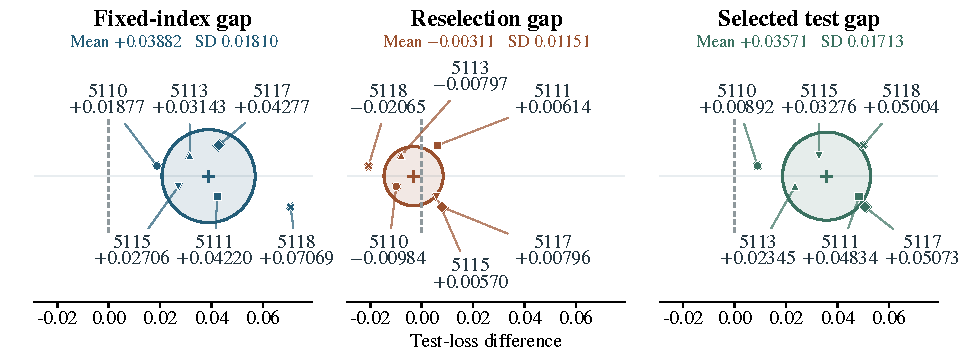
\includegraphics[width=0.96\linewidth]{nanogpt_checkpoint_gaps.pdf}
\caption{Test-loss gaps for six groups with higher selected loss and a changed index. Crosses mark means, and circle radii are one sample SD. Labels give the seed and its signed horizontal coordinate. Vertical offsets separate points. Sample variances from left to right are \(3.28\), \(1.32\), and \(2.93\) in units of \(10^{-4}\).}
\label{fig:checkpoint-gaps}
\end{figure}
\endgroup

The fixed-index test loss rose in all six groups. Reselection reduced test loss in three and increased it in three, offsetting \(0.00311\) on average. The local gradient alignment remains unmeasured.
}
  {\paragraph{Checkpoint follow-up.}
Eight seed groups had higher selected test loss with exchange. Two kept the same selected index, with gaps \(+0.01162\) and \(+0.00037\). For the six that changed index, I also scored the exchange checkpoint at the independent arm's chosen index on the same 32 test minibatches, using 192 additional test forwards and zero gradient evaluations.

Let \(i\) and \(j\) be the validation-selected indices in the exchange (\(S\)) and independent (\(I\)) runs. With \(L\) denoting test loss, Figure~\ref{fig:checkpoint-gaps} shows the two terms below and their sum.
\[
 L_S(i)-L_I(j)
 =\underbrace{L_S(j)-L_I(j)}_{\text{fixed-index gap}}
 +\underbrace{L_S(i)-L_S(j)}_{\text{reselection gap}}.
\]

\begingroup
\setlength{\intextsep}{5pt}
\begin{figure}[!ht]
\centering
\setlength{\abovecaptionskip}{3pt}
\small
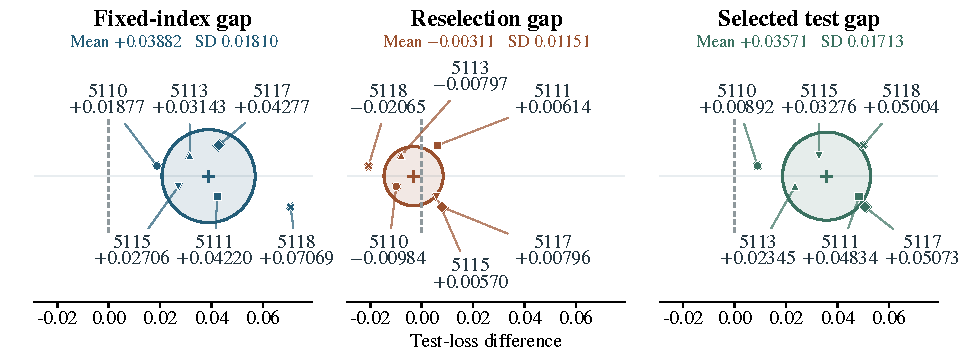
\includegraphics[width=0.96\linewidth]{nanogpt_checkpoint_gaps.pdf}
\caption{Test-loss gaps for six groups with higher selected loss and a changed index. Crosses mark means, and circle radii are one sample SD. Labels give the seed and its signed horizontal coordinate. Vertical offsets separate points. Sample variances from left to right are \(3.28\), \(1.32\), and \(2.93\) in units of \(10^{-4}\).}
\label{fig:checkpoint-gaps}
\end{figure}
\endgroup

The fixed-index test loss rose in all six groups. Reselection reduced test loss in three and increased it in three, offsetting \(0.00311\) on average. The local gradient alignment remains unmeasured.
}
\end{sloppypar}

\clearpage
\subsection{Training trajectories and final evaluation}

\begin{figure}[!ht]
\centering
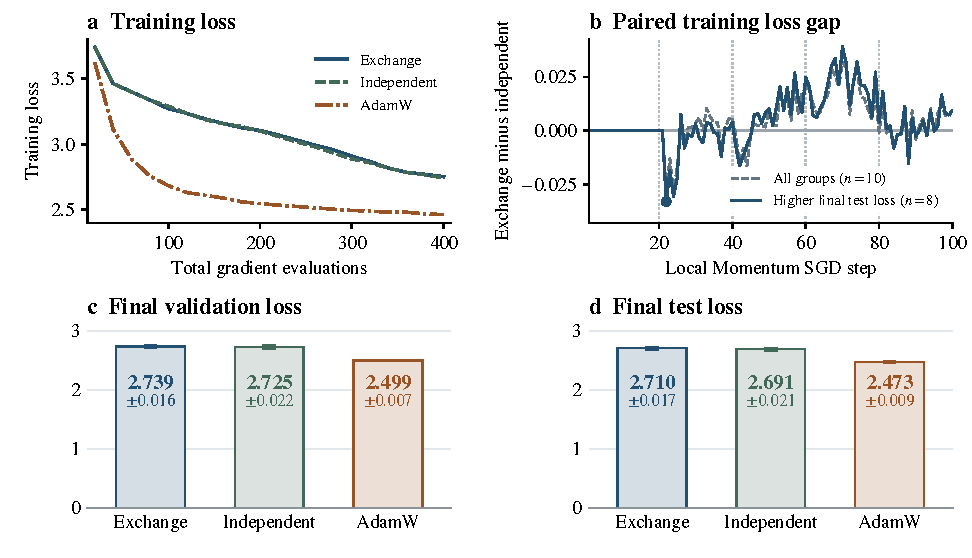
\includegraphics[width=0.98\linewidth]{nanogpt_loss_comparison.pdf}
\caption{Training and held-out losses from ten paired seed groups. \textbf{a} Training loss averaged over successive blocks of 20 gradient evaluations, pooling replicas within each group. \textbf{b} Mean paired training loss differences at each local step. Dotted lines mark the steps followed by a swap. The dot marks the first loss that can reflect the swap, and the eight-group curve is selected by final test deterioration. \textbf{c, d} Final losses of the validation-selected checkpoint in each arm, measured on 32 validation or test minibatches. Bars show means. Whiskers and the labels give \(\pm1\) sample SD across seeds.}
\label{fig:nanogpt-losses}
\end{figure}

\paragraph{Training trajectory.}
Figure~\ref{fig:nanogpt-losses} compares training at equal gradient budgets. At step 22, the first observation after an update used swapped velocity, the matched training minibatch loss was lower for \(32/40\) replicas across all ten groups, with mean difference \(-0.02848\). The mean gap over steps 62--80 was \(+0.01661\), after several exchanges. In the eight groups with worse final test loss, the corresponding means were \(-0.03307\) and \(+0.01985\). The late comparison includes the history of earlier swaps.

At a common parameter vector \(\theta\) and minibatch loss \(f\), the retained velocity \(a\) and incoming velocity \(b\) give trial displacements \(d_w=\mu w-\eta g\), where \(g\) is the clipped gradient. If \(f\) is differentiable at \(\theta\), a first-order expansion with \(\tilde g=\nabla f(\theta)\) gives
\[
f(\theta+\varepsilon d_b)-f(\theta+\varepsilon d_a)
=\varepsilon\,\mu\tilde g^\top(b-a)+o(\varepsilon).
\]
The term can have either sign. The early gain on a training minibatch can fade as the iterates visit different points and receive different gradients. Proposition~\ref{prop:quadratic-exchange} shows how a conservative swap can worsen both subsequent losses even on a stable quadratic. The recorded norms and hashes leave the sign of the inner product at individual NanoGPT swaps undetermined.

\paragraph{Final evaluation.}
Mean selected validation losses were \(2.73885\) for exchange, \(2.72517\) for independent Momentum SGD, and \(2.49947\) for AdamW. In the six worse test cases that switched replica, fixed-index test loss rose by \(0.03882\) on average and reselection offset \(0.00311\). Together with the later training gap, this points to the changed trajectory as the main observed source of the endpoint difference in these cases. AdamW also led plain Momentum in the separate single-replica comparison at 400 steps per method. Weight decay was zero in both comparisons, so they do not isolate an effect of decoupled decay.

\clearpage
\section{Momentum balance and limits of exchange}
\label{sec:balance}

\paragraph{Balance between swaps.}
For unit-mass replicas, write \(P_t^{\pm}=\sum_i u_{i,t}^{\pm}\) and \(K_t^{\pm}=\tfrac12\sum_i\|u_{i,t}^{\pm}\|^2\). Summing the SGD update \(u_{i,t+1}^{-}=\mu u_{i,t}^{+}-\eta g_{i,t+1}\) and expanding its squared norm give
\begin{align*}
P_{t+1}^{-}-P_t^{+}
  &= (\mu-1)P_t^{+}-\eta\sum_i g_{i,t+1},\\
K_{t+1}^{-}-K_t^{+}
  &= -(1-\mu^2)K_t^{+}
     -\mu\eta\sum_i\langle u_{i,t}^{+},g_{i,t+1}\rangle
     +\tfrac{\eta^2}{2}\sum_i\|g_{i,t+1}\|^2 .
\end{align*}
For \(0\le\mu<1\), the first term in the energy balance represents dissipation. The mixed term can add or remove kinetic energy depending on the velocity's alignment with the clipped gradient.

\paragraph{What the proofs establish.}
Theorem~\ref{thm:bounce} classifies the undamped linearized bounce, including linear growth at the boundary. For native momentum and trial reflection, Theorem~\ref{thm:momentum-rate} derives an \(O(1/T)\) bound on the average squared gradient with exact gradients and a corresponding error term under gradient noise. The condition \(\eta L<1-\mu^2\) is sufficient for this bound. For the Adam-family extension, Theorem~\ref{thm:adam-guard} gives a rate for a candidate checked against a smooth upper model with a gradient-step fallback. These rates concern stationarity on the optimized objective. The NanoGPT runs used clipped gradients and did not certify \(L\), and Adam-family population exchange with the safeguard remains a proposed method.

\paragraph{What remains to prove.}
In a double well, a particle crossing a barrier of value \(f_s\) needs mechanical energy at least \(g(f_s-f_\star)\) at the crossing, since \(z\ge f(x)\). A comparative escape theorem would identify a region of starting states trapped by the base method and show that a reachable conservative transfer sends a particle over the barrier and into a trapping region of the better well. For incumbent protection, a finite-horizon theorem would bound the nonlinear remainder at each bounce and track contact-time error, damping and any later impulses to keep saved losses below the departure threshold.

\paragraph{When to exchange in a gradient method.}
For the same optimizer state, let \(y\) be the base step endpoint and \(\Delta\) the change in that step from an exchange. The smoothness estimate in Appendix~\ref{app:adam} gives a sufficient test for a lower next loss,
\(\nabla f(y)^\top\Delta+(L/2)\|\Delta\|^2<0\).
Its gradient can cost an extra evaluation and the local curvature bound must be justified. A budget-matched improvement theorem would need a bound on the cumulative gain after accounting for these costs and for changes in subsequent gradients. An explanation of held-out performance also needs evidence about the training trajectory and its generalization.

\paragraph{Benchmarks for follow-up.}
COCO/BBOB offers separable and nonseparable Rastrigin functions and \mbox{Lunacek} bi-Rastrigin \cite{bbob}. These tasks would test escape across more minima and coupled directions. An initial comparison could use the external-displacement wrapper with common starts and paid gradient queries. Using the gravity solver would also require locating the first wall contact along a path, with every probe charged. \mbox{DeepOBS} provides a 100-dimensional noisy quadratic and a compact CIFAR-10 CNN \cite{deepobs}. The quadratic would test exchange alignment under controlled gradient noise. The CNN would test whether early training gains survive to validation and test beyond language modeling, with independent replicas and the unmodified base optimizer as controls.

\clearpage
\begin{thebibliography}{14}
\setlength{\itemsep}{0pt}
\bibitem{polyak} B. T. Polyak. Some methods of speeding up the convergence of iteration methods. \emph{USSR Computational Mathematics and Mathematical Physics}, 4(5), 1--17, 1964. \href{https://doi.org/10.1016/0041-5553(64)90137-5}{DOI}.
\bibitem{pytorchsgd} PyTorch. \href{https://docs.pytorch.org/docs/2.10/generated/torch.optim.SGD.html}{SGD documentation}, version 2.10.
\bibitem{easgd} S. Zhang, A. Choromanska, and Y. LeCun. Deep learning with elastic averaging SGD. \emph{Advances in Neural Information Processing Systems}, 28, 2015. \href{https://proceedings.neurips.cc/paper/2015/hash/d18f655c3fce66ca401d5f38b48c89af-Abstract.html}{Proceedings}.
\bibitem{dullin} H. R. Dullin. Linear stability in billiards with potential. \href{https://arxiv.org/abs/chao-dyn/9612023}{arXiv:chao-dyn/9612023}, 1996.
\bibitem{restart} B. O'Donoghue and E. Cand\`es. Adaptive restart for accelerated gradient schemes. \href{https://arxiv.org/abs/1204.3982}{arXiv:1204.3982}, 2012.
\bibitem{adamw} I. Loshchilov and F. Hutter. Decoupled weight decay regularization. \href{https://arxiv.org/abs/1711.05101}{arXiv:1711.05101}, 2017.
\bibitem{adam} D. P. Kingma and J. Ba. Adam: A method for stochastic optimization. \href{https://arxiv.org/abs/1412.6980}{ICLR}, 2015.
\bibitem{adamcounter} S. J. Reddi, S. Kale, and S. Kumar. On the convergence of Adam and beyond. \href{https://arxiv.org/abs/1904.09237}{ICLR}, 2018.
\bibitem{nanogpt} A. Karpathy. \href{https://github.com/karpathy/nanoGPT/tree/3adf61e154c3fe3fca428ad6bc3818b27a3b8291}{nanoGPT}, source revision \texttt{3adf61e}, MIT license.
\bibitem{data} A. Karpathy. \href{https://github.com/karpathy/char-rnn/blob/master/data/tinyshakespeare/input.txt}{Tiny Shakespeare}, text distribution in the char-rnn repository.
\bibitem{bbob} COCO. \href{https://coco-platform.org/testsuites/bbob/overview.html}{The BBOB test suite and function definitions}.
\bibitem{deepobs} F. Schneider, L. Balles, and P. Hennig. DeepOBS: A deep learning optimizer benchmark suite. \href{https://arxiv.org/abs/1903.05499}{ICLR}, 2019.
\end{thebibliography}
\appendix
\fontsize{9.5}{11.4}\selectfont
\setlength{\parskip}{3pt}
\setlength{\abovedisplayskip}{6pt plus 2pt minus 2pt}
\setlength{\belowdisplayskip}{6pt plus 2pt minus 2pt}
\setlength{\abovedisplayshortskip}{3pt plus 1pt}
\setlength{\belowdisplayshortskip}{4pt plus 1pt minus 1pt}
\section{Additional comparisons and reproducibility}
\label{app:details}

\paragraph{Discretization and dimension.}
Across 240 single-trajectory tests from \(100\) to \(10^5\) dimensions, active reflection overflowed in one \(10^5\)-dimensional Rosenbrock run. A separate fixed-time hybrid run hit a contact-event cap at \(h=0.05\). The fixed-time cases completed at \(h=0.025\) and \(0.0125\) with higher query cost, and the runner was repaired to retain failures and resume. In a separate 1,500-query comparison on 10D Rosenbrock, median normalized best-loss gaps were \(7.17\times10^{-8}\) for Momentum, \(1.85\times10^{-7}\) for Adam, and \(1.745\times10^{-2}\) for pure gravity. The four-particle matched scattering comparisons were two-dimensional.

\paragraph{Damping and handoff controls.}
On Rosenbrock, ramped and constant stronger damping gave \(18/20\) and \(19/20\) final hits. With a shared collision prefix, decoupling reduced the quadratic median final normalized gap from \(0.04624\) to \(0.00218\), while Rosenbrock final hits moved from \(18/20\) to \(17/20\). In a distinct held-out double-well test with a handoff budget fixed on development seeds, normal and random scattering reached the target in \(14/20\) and \(16/20\). Four-start GD and Momentum each reached \(0/20\) from the common poor-basin starts, and each reached \(20/20\) on quadratic and Rosenbrock.

\paragraph{Selective intervention.}
In a constructed double-well launch study, 24 seeds supplied 168 matched conditions. Bounding loss at the first three saved points preserved all 120 departures prevented by exact prediction and reduced prediction queries from 612 to 533. A paired follow-up on the same launches checked the fourth point selectively and prevented seven additional departures for 24 additional prediction queries. Across both comparisons, no transfer occurred in the 27 safe controls. The follow-up reused 161 trajectories and executed seven new branches. Fourteen cases still departed at some saved time, and all 168 were within the threshold at the end. These counts describe the chosen launch distribution.

\paragraph{External-impulse trial.}
Three seeds per method, with 1,200 forward-equivalent units allowed. A training update cost three units and a diagnostic forward cost one. The random and preview variants had identical reported outcomes.
\begin{center}
\small
\begin{tabular}{@{}lrr@{}}
\toprule
Optimizer and wrapper & Mean final test loss & Training updates\\
\midrule
Momentum SGD & 2.53177 & 400\\
Momentum SGD + random / preview impulse & 2.55027 & 386\\
Adam and AdamW, each & 2.50082 & 400\\
AdamW + random / preview impulse & 2.50923 & 386\\
\bottomrule
\end{tabular}
\end{center}
\section{Computational cost and records}
\label{app:algorithms}

\paragraph{Gravity search (Algorithm~\ref{alg:gravity}).}
Let \(d\) be the horizontal dimension and \(P\) the particle count. Over \(S\) completed observation intervals, let \(A\) count the passes through the contact-search loop and \(E\) count contacts resolved. Each pass resolves at least one contact or finishes the interval, so \(A\le S+E\).

\begin{center}
\small
\begin{tabular}{@{}p{0.41\linewidth}ll@{}}
\toprule
Operation & Number of calls or operations & Cost per operation\\
\midrule
Advance, damp, or bookkeep one particle & \(O((A+S+1)P)\) & \(O(d)\)\\
Test a pair for collision or overlap & \(O((A+S+1)P^2)\) & \(O(d)\)\\
Find the next wall root for one particle & \(AP\) & \(C_{\rm wall}\)\\
Apply a contact update & \(E\) & \(O(d)\)\\
Evaluate loss or gradient outside wall search & \(Q_f,\ Q_g\) & \(C_f,\ C_g\)\\
\bottomrule
\end{tabular}
\end{center}
The time bound is the sum of the rowwise products. \(C_{\rm wall}\) includes the path query and root solving. \(Q_f,Q_g\) count feasibility, contact, and observation queries outside the search. A full pass with pair contact enabled tests \(\binom{P}{2}\) candidate collisions. This is where the quadratic cost in \(P\) arises.

\paragraph{Training and evaluation (Algorithms~\ref{alg:damping}--\ref{alg:external}).}
Let \(P\) be the replica count and \(d\) the number of model parameters per replica. One minibatch gradient costs \(C_\nabla\), including the forward and backward passes, and one evaluation forward costs \(C_{\rm fwd}\). For \(G\) gradients and \(F\) evaluation forwards, the base time is \(O(G(C_\nabla+d)+FC_{\rm fwd})\), including \(O(d)\) optimizer work per update. Let \(T\) be the updates per replica, \(V\) the validation batches per candidate, \(W\) the test batches for the chosen model, and \(J\) the number of pair swaps.

\begin{center}
\small
\begin{tabular}{@{}lllp{0.42\linewidth}@{}}
\toprule
Algorithm & Gradients \(G\) & Eval.\ forwards \(F\) & Added work over the base optimizer\\
\midrule
\ref{alg:damping}. Damping / reset & \(T\) & \(W\) & \(O(Td)\) for norm checks and buffer scaling\\
\ref{alg:swap}. Native exchange & \(PT\) & \(PV+W\) & \(O(Jd)\) for the audited swaps\\
\ref{alg:external}. External exchange & \(PT\) & \(PV+W\) & \(O(PTd+Jd)\) for auxiliary updates, checks, and swaps\\
\bottomrule
\end{tabular}
\end{center}

In the primary NanoGPT comparison, \(P=4\), \(T=100\), and \(V=W=32\). Per seed, each Momentum SGD arm uses 400 gradients, 128 validation forwards, and 32 test forwards. The exchange arm adds eight audited pair swaps. Hashing and conservation checks scan the parameter and velocity buffers, giving the \(O(d)\) cost per audited swap. The safeguard reuses the current gradient. Any search used to supply impulses adds its own oracle cost.

The model parameters and optimizer buffers occupy \(O(Pd)\) live space. Algorithm~\ref{alg:external} adds \(O(Pd)\) auxiliary storage. These counts exclude network activations and saved records.

\paragraph{Reproducibility.}
The experiment record includes paired seeds, source snapshots, trajectories, event logs, and query counts. The NanoGPT record includes initial-state hashes, final checkpoints, selected replica indices, and individual minibatch scores for the checkpoint follow-up.

\clearpage
\section{Stability and rates for the original methods}
\label{app:rates}

\paragraph{Formal verification.}
Lean 4 verifies the exact-gradient rates in Theorem~\ref{thm:momentum-rate}, the pathwise stationarity bound, and the centered-noise bounds for finite sampling. It also verifies the two stationarity bounds and the geometric loss bounds for the descent safeguard in Appendix~\ref{app:adam}.

\paragraph{Energy accounting for gravity search.}
Consider exact feasible trajectories of Algorithm~\ref{alg:gravity} with finitely many resolved events on the interval under study, unit masses, common gravity \(g>0\), elastic wall impacts, conservative pair collisions, and the damping ticks specified below. Assume \(f\ge f_\star\) and set
\[
\mathcal E(t)=\sum_{i=1}^{P}\left(\tfrac12\|V_i(t)\|^2+g(z_i(t)-f_\star)\right).
\]
In flight, the kinetic and potential derivatives are \(-gV_{i,z}\) and \(gV_{i,z}\), respectively. Contact positions are fixed at impact, and both kinds of collision preserve total kinetic energy. At tick \(t_j\), scaling velocities by \(0\le\beta_j\le1\) removes \((1-\beta_j^2)K_j^-\), where \(K_j^-\) is the total kinetic energy just before the tick. Summing the jumps and using \(z_i\ge f(x_i)\ge f_\star\) gives
\[
\mathcal E(t)+\sum_{t_j\le t}(1-\beta_j^2)K_j^-=\mathcal E(0^-),
\qquad
0\le f(x_i(t))-f_\star\le\mathcal E(0^-)/g.
\]
If \(\beta_j\le\bar\beta<1\) at \(N\ge1\) ticks, then the balance gives \((1-\bar\beta^2)\sum_{j=1}^N K_j^-\le\mathcal E(0^-)\). Bounding the smallest \(K_j^-\) by its average yields \(\min_{1\le j\le N}K_j^-\le \mathcal E(0^-)/[N(1-\bar\beta^2)]\).

\paragraph{What the bounds measure.}
If \(f(x)-f_\star\ge (m/2)\|x-x_\star\|^2\) globally for some \(m>0\), then \(\|x_i(t)-x_\star\|^2\le 2\mathcal E(0^-)/(gm)\). For the undamped linearized orbit of Theorem~\ref{thm:bounce}, the sharper horizontal bound is \(x_n^2\le Q(x_0,x_0+Tu_0)/(1-\tau^2/4)\), where \(T\) is the orbit's flight time. Its loss error is \(\kappa x_n^2/2\). The invariant \(Q\) stays positive for a nonzero perturbation, so such a perturbation cannot converge to the zero phase state. The damping rate controls kinetic energy at the ticks. A stationary-point rate is available if the search hands its best point to deterministic gradient descent. After \(N\) such refinement steps with step \(1/L\) on a lower-bounded \(L\)-smooth objective, the descent inequality in Theorem~\ref{thm:adam-guard} gives \(\min_{k<N}\|\nabla f(x_k)\|^2\le 2L(f(x_0)-f_\star)/N\), where \(x_0\) is the handoff point. This is a refinement option distinct from the gravity-only runs.

\paragraph{Trial reflection in displacement units.}
For the implemented trial reflection, physical velocity \(v\) corresponds to stored displacement \(u=hv\). With gradient scale \(\gamma\), set \(\eta=\gamma h^2\) and momentum \(\mu=\beta\). The trial is \(s=\mu u-\eta\nabla f(x)\). A round is flagged when \(s\) points uphill above the cosine threshold and the normalized trial loss increase exceeds its threshold. Once the flag persists for the required number of consecutive rounds, reflect \(s\) about the gradient normal. Otherwise keep \(s\). Advance by and store the resulting displacement. The next theorem covers any such trigger that reflects only when the trial has positive inner product with the true gradient.

\paragraph{Velocity bounds at the tested settings.}
In the momentum updates below, if \(\|G_{i,t}\|\le C\), the stacked displacement satisfies \(\|u_{t+1}\|\le\mu\|u_t\|+\eta C\sqrt P\). This follows from the triangle inequality and because the applied reflection or exchange cannot increase the summed squared step lengths. Iterating gives \(\|u_t\|\le\mu^t\|u_0\|+\eta C\sqrt P(1-\mu^t)/(1-\mu)\). For the four-replica NanoGPT settings this gives \(\|u_t\|\le6\) in parameter units from \(u_0=0\).

\clearpage
\begin{theorem}[Rates for momentum, reflection, and exchange]\label{thm:momentum-rate}
Let \(f\) be \(L\)-smooth on \(\mathbb R^d\), \(L>0\), and \(f\ge f_\star\). For each of \(P\) replicas form \(s_{i,t}=\mu a_{i,t}u_{i,t}-\eta G_{i,t}\), where \(0\le\mu<1\), \(0\le a_{i,t}\le1\), and
\(\eta>0\), \(\eta L<1-\mu^2\). Write \(\delta=1-\eta L-\mu^2>0\). Use one of the following updates.
\begin{itemize}\setlength{\itemsep}{0pt}
\item For native Momentum SGD, let \(d_{i,t}=s_{i,t}\).
\item For deterministic trial reflection, let \(G_{i,t}=\nabla f(x_{i,t})\). When \(G_{i,t}^\top s_{i,t}>0\), one may set \(d_{i,t}=s_{i,t}-(1+e)(s_{i,t}^\top n)n\) for \(0\le e\le1\) and \(n=G_{i,t}/\|G_{i,t}\|\). In other rounds let \(d_{i,t}=s_{i,t}\).
\end{itemize}
Set \(x_{i,t+1}=x_{i,t}+d_{i,t}\). Store the displacements as the new \(u_{i,t+1}\), allowing any post-step exchange with \(\sum_i\|u_{i,t+1}\|^2\le\sum_i\|d_{i,t}\|^2\). In particular, Algorithm 3's swaps give equality. Define
\[
\Psi_t=\sum_i(f(x_{i,t})-f_\star)+c\sum_i\|u_{i,t}\|^2,\qquad
c=\frac{1-\eta L}{2\eta}.
\]
For \(P,T\ge1\) and exact gradients, the average squared gradient through \(T\) updates is at most \(2\Psi_0/(\eta PT)\). If \(f\) also satisfies \(\|\nabla f(x)\|^2\ge 2m(f(x)-f_\star)\) for \(0<m\le L\), then
\[
\Psi_T\le (1-r)^T\Psi_0,\qquad
r=\min\{\eta m,\ \delta/(1-\eta L)\}.
\]
For native momentum with \(G_{i,t}=\nabla f(x_{i,t})+\xi_{i,t}\), the pathwise bound on the average squared true gradient is
\[
\frac{2\Psi_0}{\eta PT}+
\left(1+\frac{2\mu^2}{\delta}\right)
\frac{\sum_{t<T}\sum_i\|\xi_{i,t}\|^2}{PT}.
\]
If the initial energy is integrable, \(u_{i,t}\) and \(a_{i,t}\) are measurable with respect to the history \(\mathcal F_t\) before drawing the batch, and
\(\mathbb E[\xi_{i,t}\mid\mathcal F_t]=0\), \(\mathbb E[\|\xi_{i,t}\|^2\mid\mathcal F_t]\le\sigma^2\),
the expected bound is \(2\mathbb E[\Psi_0]/(\eta PT)+\sigma^2\).
\end{theorem}

\begin{proof}
\textit{One-step bound.} Write \(g=\nabla f(x)\), \(p=\mu a u\), and \(s=p-\eta(g+\xi)\) at one replica. Smoothness bounds the loss change by \(g^\top d+(L/2)\|d\|^2\). Reflection reverses and scales the positive component along \(n\), giving \(g^\top d\le g^\top s\) and \(\|d\|\le\|s\|\). Both inequalities also hold for \(d=s\). With \(c>0\), the post-step exchange bound lets us charge the next kinetic term as \(c\sum_i\|d_{i,t}\|^2\). Since \(L/2+c=1/(2\eta)\), the contribution per replica is bounded by
\[
g^\top s+\frac{\|s\|^2}{2\eta}
=\frac{\|p\|^2}{2\eta}-\frac{\eta}{2}\|g\|^2
 +\frac{\eta}{2}\|\xi\|^2-p^\top\xi .
\]
Sum this bound and subtract \(c\sum_i\|u_{i,t}\|^2\). Using \(\|p\|^2\le\mu^2\|u\|^2\) leaves
\[
\Psi_{t+1}-\Psi_t
\le\sum_i\left[-\frac{\delta}{2\eta}\|u_{i,t}\|^2
-\frac{\eta}{2}\|\nabla f(x_{i,t})\|^2
+\frac{\eta}{2}\|\xi_{i,t}\|^2-p_{i,t}^\top\xi_{i,t}\right].
\]
\textit{Exact gradients.} Telescope with \(\xi=0\) and use \(\Psi_T\ge0\). The sum of squared gradients is finite, so each replica's gradient tends to zero. Also \(\sum_i\|u_{i,t}\|^2\le\Psi_0/c\), and bounded objective sublevels give bounded positions. Under gradient dominance the two negative terms remove at least \(\eta m\) times the loss gap and \(\delta/(1-\eta L)\) times the kinetic term, giving the claimed contraction.

\textit{Gradient errors.} Young's inequality gives \(-p^\top\xi\le\delta\|u\|^2/(4\eta)+(\eta\mu^2/\delta)\|\xi\|^2\). The first term absorbs only half the negative velocity term, so telescoping gives the pathwise bound. For the expected bound, that same pathwise estimate and the second moment bound ensure finite expected energy at every finite step. Since \(p\) is measurable before the batch, \(\mathbb E[p^\top\xi\mid\mathcal F_t]=0\). Take expectations in the one-step bound and telescope.
\end{proof}

The pathwise error includes bias from clipping and allows Algorithm 2's current-batch trigger. The sharper noise bound needs predictability and an unbiased gradient. Independent batch averaging without clipping reduces \(\sigma^2\) inversely with batch size. The sufficient step restriction uses the objective's smoothness constant. The NanoGPT comparison did not certify \(L\). Plain SGD is the case \(\mu=0\), with no native momentum to transfer.

\paragraph{Loss under gradient dominance and centered noise.}
Under both of these hypotheses of Theorem~\ref{thm:momentum-rate}, the one-step estimate gives \(\mathbb E\Psi_{t+1}\le(1-r)\mathbb E\Psi_t+\eta P\sigma^2/2\). Iterating the geometric sum yields
\[
\mathbb E\Psi_T\le(1-r)^T\mathbb E[\Psi_0]+
  \frac{\eta P\sigma^2}{2r}\bigl(1-(1-r)^T\bigr).
\]

\clearpage
\section{Stability and convergence of the external exchange}
\label{app:adam}

\paragraph{Size of the auxiliary displacement.}
In Algorithm~\ref{alg:external}, the stacked auxiliary displacement \(q_t\) and impulses \(J_t\) satisfy \(q_{t+1}=\rho S_t(q_t+J_t)\), where \(S_t\) permutes replica blocks and \(0\le\rho<1\). The permutation preserves the norm, so \(\|q_{t+1}\|\le\rho(\|q_t\|+\|J_t\|)\). Iteration gives
\[
\|q_t\|\le \rho^t\|q_0\|+\sum_{k=0}^{t-1}\rho^{t-k}\|J_k\| .
\]
Thus the displacement decays geometrically after the last impulse. To bound its squared size over a run, use
\[
(1-\rho)\rho^2(a+b)^2\le (1-\rho)\rho a^2+\rho^2 b^2,
\qquad a=\|q_t\|,\quad b=\|J_t\| .
\]
The difference is \(\rho((1-\rho)a-\rho b)^2\ge0\). Summing the resulting bound on \((1-\rho)\|q_{t+1}\|^2\) and moving the repeated terms to the left gives
\[
\sum_{t=1}^{T}\|q_t\|^2\le
\frac{\rho}{1-\rho}\|q_0\|^2+
\frac{\rho^2}{(1-\rho)^2}\sum_{k=0}^{T-1}\|J_k\|^2.
\]

\paragraph{Effect on the unguarded candidate loss.}
At a fixed optimizer state, let \(y=x+b\) be the base step's endpoint and \(q\) the added displacement. If \(f\) is \(L\)-smooth, integrating \(\nabla f(y+s q)^\top q\) from \(s=0\) to \(1\) gives
\[
\big|f(y+q)-f(y)-\nabla f(y)^\top q\big|\le \tfrac L2\|q\|^2 .
\]
The bound on \(\sum_{t=1}^{T}\|q_t\|^2\) controls the sum of these quadratic remainders. The first-order term can have either sign, and the adaptive moments at later steps depend on the parameter trajectory.

\begin{theorem}[Stationarity under the descent safeguard]\label{thm:adam-guard}
Let \(f\ge f_\star\) be \(L\)-smooth on \(\mathbb R^d\), \(L>0\), and use guarded mode with \(0<\eta\le1/L\). For any replica and \(T\ge1\), suppose \(\|G_t-\nabla f(x_t)\|\le\varepsilon_t\). For exact gradients set \(\varepsilon_t=0\). Then
\[
\begin{aligned}
\min_{0\le t<T}\|\nabla f(x_t)\|^2
 &\le \frac{2(f(x_0)-f_\star)}{\eta T}
 &&\text{with exact gradients},\\
\min_{0\le t<T}\|\nabla f(x_t)\|^2
 &\le \frac{8(f(x_0)-f_\star)}{\eta T}
      +\frac{34}{T}\sum_{t<T}\varepsilon_t^2
 &&\text{with bounded gradient error}.
\end{aligned}
\]
If \(f\) also satisfies \(\|\nabla f(x)\|^2\ge2m(f(x)-f_\star)\) for \(0<m\le L\), exact gradients give \(f(x_T)-f_\star\le(1-\eta m)^T(f(x_0)-f_\star)\).
\end{theorem}

\begin{proof}
\textit{Fallback and descent.} For \(d=-\eta G_t\), the first test has left side \(-\eta(1-\eta L/2)\|G_t\|^2\), which meets the required decrease since \(\eta L\le1\). The second holds because \(\|d\|=\eta\|G_t\|\). Both branches therefore obey
\[
f(x_t+d)-f(x_t)
\le G_t^\top d+\tfrac L2\|d\|^2+\varepsilon_t\|d\|
\le-\tfrac\eta2\|G_t\|^2+2\eta\varepsilon_t\|G_t\|.
\]
\textit{Rates.} For exact gradients, sum the inequality or apply gradient dominance at each step for geometric decrease. With error, use Young's inequality and then \(\|\nabla f(x_t)\|^2\le2\|G_t\|^2+2\varepsilon_t^2\).
\[
-\tfrac12\|G_t\|^2+2\varepsilon_t\|G_t\|
\le -\tfrac14\|G_t\|^2+4\varepsilon_t^2
\le -\tfrac18\|\nabla f(x_t)\|^2+\tfrac{17}{4}\varepsilon_t^2 .
\]
Multiply by \(\eta\), sum over \(t<T\), and use \(f(x_T)\ge f_\star\). The minimum is bounded by the resulting average.
\end{proof}

With exact gradients the loss does not increase, bounded sublevels give bounded iterates, and summability of the squared gradients implies \(\nabla f(x_t)\to0\). If \(f\) is \(m\)-strongly convex, then \(\|x_T-x_\star\|^2\le 2(f(x_T)-f_\star)/m\), so the geometric loss rate bounds the parameter error. With gradient dominance and \(\varepsilon_t\le\bar\varepsilon\), the noisy one-step loss-gap bound has contraction factor \(1-\eta m/4\) and additive term \(17\eta\bar\varepsilon^2/4\). Its limiting upper bound is \(17\bar\varepsilon^2/m\).

\end{document}
